\newcommand{\proseA}{We study the problem of estimating a parameter $\theta \in \mathbb{R}^d$ from noisy observations $y_i = \langle x_i, \theta\rangle + \varepsilon_i$, where the noise $\varepsilon_i$ is independent and sub-Gaussian with variance proxy $\sigma^2$. Throughout, $\|\cdot\|$ denotes the Euclidean norm and $n$ the number of samples. The estimator we analyse is simple to state and cheap to compute, and its risk can be bounded in terms of $d/n$ alone.}
\newcommand{\proseB}{The bound is tight up to constants: a matching lower bound follows from Fano's inequality applied to a packing of the unit sphere. When the design is well conditioned, that is $\lambda_{\min}(X^\top X) \geq c\, n$, the dependence on the dimension cannot be improved, and the rate $\sigma^2 d / n$ is attained by ordinary least squares as well as by the regularised estimator for small $\lambda$.}
\newcommand{\proseC}{Combining the two displays and taking expectations gives the claim. Note that the constant does not depend on $T$, which is what allows the horizon to be chosen adaptively; the same argument applies verbatim to the stochastic setting once the gradients are replaced by their unbiased estimates $g_t$ with $\mathbb{E}[g_t] = \nabla f(x_t)$.}

\section{Introduction}
\proseA

\proseB
The empirical risk of a predictor $f$ is
\begin{equation}\label{eq:risk}
\widehat{R}(f) = \frac{1}{n}\sum_{i=1}^{n} \ell\bigl(f(x_i), y_i\bigr),
\end{equation}
and its population counterpart is $R(f) = \mathbb{E}[\ell(f(x),y)]$. We write $f^\star$ for a minimiser of $R$ over the class $\mathcal{F}$.

\proseC

\section{Main results}
\proseA
Expanding the square, the update can be written over several lines as
\begin{align}
\|x_{t+1} - x^\star\|^2 &= \|x_t - \eta g_t - x^\star\|^2 \label{eq:a1}\\
&= \|x_t - x^\star\|^2 - 2\eta \langle g_t, x_t - x^\star\rangle + \eta^2 \|g_t\|^2 \label{eq:a2}\\
&\leq \|x_t - x^\star\|^2 - 2\eta \bigl(f(x_t) - f(x^\star)\bigr) + \eta^2 G^2. \label{eq:a3}
\end{align}
Summing over $t$ and rearranging, we obtain an unnumbered bound
\[
\frac{1}{T}\sum_{t=1}^{T} f(x_t) - f(x^\star) \leq \frac{\|x_1 - x^\star\|^2}{2\eta T} + \frac{\eta G^2}{2}.
\]
\proseB

\begin{theorem}\label{thm:main}
Let $f$ be convex and $G$-Lipschitz on a domain of diameter $D$. With step size $\eta = D/(G\sqrt{T})$, the averaged iterate $\bar{x}_T$ satisfies
\begin{equation}\label{eq:thm}
\mathbb{E}\, f(\bar{x}_T) - f(x^\star) \leq \frac{D G}{\sqrt{T}}.
\end{equation}
Moreover, for every $\delta \in (0,1)$, with probability at least $1-\delta$,
\[
f(\bar{x}_T) - f(x^\star) \leq \frac{DG}{\sqrt{T}} \left(1 + \sqrt{2\log(1/\delta)}\right).
\]
\end{theorem}

\begin{proof}
\proseC
The martingale differences are bounded, so Azuma's inequality gives
\begin{equation*}
\Pr\Bigl[\,\sum_{t=1}^{T} Z_t \geq s\Bigr] \leq \exp\Bigl(-\frac{s^2}{2 T D^2 G^2}\Bigr). \qedhere
\end{equation*}
\end{proof}

\begin{figure}[t]
\centering
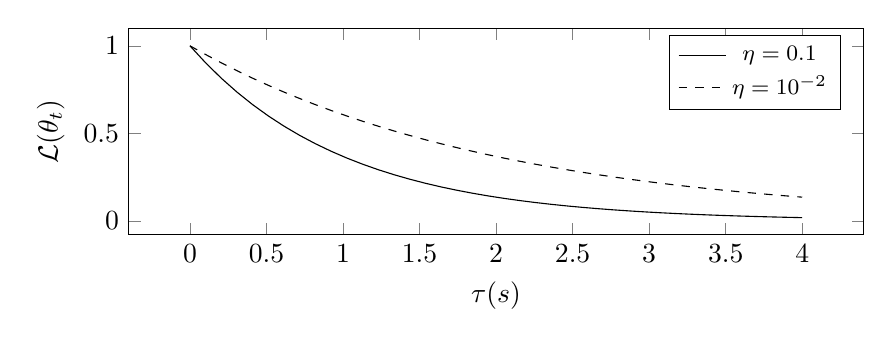
\begin{tikzpicture}
\begin{axis}[width=0.9\linewidth, height=4.2cm, xlabel={$\tau(s)$}, ylabel={$\mathcal{L}(\theta_t)$}, legend style={font=\footnotesize}, legend pos=north east]
\addplot[domain=0:4, samples=40] {exp(-x)};
\addlegendentry{$\eta = 0.1$}
\addplot[domain=0:4, samples=40, dashed] {exp(-0.5*x)};
\addlegendentry{$\eta = 10^{-2}$}
\end{axis}
\end{tikzpicture}
\caption{Training loss $\mathcal{L}(\theta_t)$ against the rescaled time $\tau(s)$ for two step sizes.}
\label{fig:loss}
\end{figure}

\section{Further displays}
\proseC
Several equations can be gathered and centred together:
\begin{gather*}
\mathcal{H}(p) = -\sum_{x} p(x) \log p(x),\\
D_{\mathrm{KL}}(p \,\|\, q) = \sum_{x} p(x) \log \frac{p(x)}{q(x)}.
\end{gather*}
A long equation is broken with \texttt{multline}:
\begin{multline}\label{eq:multline}
\mathcal{J}(\theta) = \mathbb{E}_{x \sim p}\bigl[\log D_\phi(x)\bigr] + \mathbb{E}_{z \sim q}\bigl[\log\bigl(1 - D_\phi(G_\theta(z))\bigr)\bigr] \\
+ \lambda\, \mathbb{E}_{\hat{x}}\Bigl[\bigl(\|\nabla_{\hat{x}} D_\phi(\hat{x})\|_2 - 1\bigr)^2\Bigr] + \mu \|\theta\|_2^2.
\end{multline}
\proseA
An equation carrying its own tag:
\begin{equation}
V^\pi(s) = \mathbb{E}_\pi\Bigl[\sum_{k=0}^{\infty} \gamma^k r_{t+k+1} \Bigm| s_t = s\Bigr] \tag{$\star$}
\end{equation}
and a piecewise definition,
\begin{equation}\label{eq:cases}
\mathrm{sign}(x) = \begin{cases} 1 & \text{if } x > 0,\\ 0 & \text{if } x = 0,\\ -1 & \text{otherwise.}\end{cases}
\end{equation}
\proseB

\begin{table}[t]
\centering
\caption{Test error (\%) of each method on three benchmarks.}
\label{tab:res}
\begin{tabular}{lccc}
\toprule
Method & $n = 10^3$ & $n = 10^4$ & $n = 10^5$ \\
\midrule
SGD & 12.4 & 8.1 & 5.3 \\
Adam & 11.9 & 7.6 & 5.0 \\
$\ell_2$-reg. & 12.0 & 7.9 & 5.1 \\
Ours ($\lambda = 0.1$) & \textbf{10.2} & \textbf{6.4} & \textbf{4.2} \\
\bottomrule
\end{tabular}
\end{table}

\section{Algorithm}
\proseA

\begin{algorithm}[t]
\caption{Projected stochastic gradient descent}
\label{alg:psgd}
\begin{algorithmic}[1]
\Require step size $\eta > 0$, horizon $T$, start $x_1 \in \mathcal{K}$
\For{$t = 1, \dots, T$}
\State sample $g_t$ with $\mathbb{E}[g_t \mid x_t] = \nabla f(x_t)$
\State $y_{t+1} \gets x_t - \eta\, g_t$
\State $x_{t+1} \gets \Pi_{\mathcal{K}}(y_{t+1})$
\EndFor
\State \Return $\bar{x}_T = \frac{1}{T}\sum_{t=1}^{T} x_t$
\end{algorithmic}
\end{algorithm}

\proseB
Matrices and aligned systems also appear in displays,
\begin{equation}\label{eq:matrix}
\begin{pmatrix} a & b \\ c & d \end{pmatrix}^{-1} = \frac{1}{ad - bc}\begin{pmatrix} d & -b \\ -c & a \end{pmatrix},
\end{equation}
\begin{align*}
\nabla_\theta \mathcal{L} &= \frac{1}{n} \sum_{i=1}^n \nabla_\theta \ell_i, &
\nabla^2_\theta \mathcal{L} &= \frac{1}{n} \sum_{i=1}^n \nabla^2_\theta \ell_i.
\end{align*}
\proseC
The integral form of the remainder is
\begin{equation}\label{eq:int}
f(y) = f(x) + \int_0^1 \bigl\langle \nabla f\bigl(x + s(y-x)\bigr),\, y - x \bigr\rangle \, ds.
\end{equation}
\proseA
